
%(BEGIN_QUESTION)
% Copyright 2007, Tony R. Kuphaldt, released under the Creative Commons Attribution License (v 1.0)
% This means you may do almost anything with this work of mine, so long as you give me proper credit

When measuring the volume of liquid stored in a vertical cylinder, the function relating liquid height ($h$) to stored liquid volume ($V$) is quite simple:

$$\includegraphics[width=15.5cm]{i02957x01.eps}$$

$$V = \pi r^2 h$$

The term $\pi r^2$ defines the cross-sectional area of the cylindrical tank, which when multiplied by the liquid height ($h$) gives an answer for volume ($V$) in cubic units.

\vskip 10pt

Calculating stored liquid volume in a {\it horizontal} cylinder is not nearly as simple.  The effective cross-sectional area of the cylinder varies with liquid height, and this variation is not linearly proportional to height.  As a result, the function relating liquid height to stored liquid volume is quite complex:

$$\includegraphics[width=15.5cm]{i02957x02.eps}$$

$$V = L \left[ (h-r) \sqrt{2hr - h^2} + r^2 \sin^{-1}{(h-r) \over r} + {\pi r^2 \over 2} \right]$$

Using this formula, calculate the amount of liquid volume stored in a horizontal cylinder with the following dimensions, assuming a liquid height ($h$) of 3 feet:

\vskip 10pt

$r$ = 5 feet

$L$ = 25 feet

\vskip 10pt

Express your answer in units of gallons.  {\it Note: the formula shown assumes the use of ``radians'' as the unit of angle measurement for the arc-sine function rather than ``degrees.''}

\underbar{file i02957}
%(END_QUESTION)





%(BEGIN_ANSWER)

$V =$ 495.4 ft$^{3}$ = 3706 gallons

\vskip 10pt

Note: if your answer is wildly in error, you might want to check to see that your calculator is set to do trigonometric functions in units of {\it radians} instead of {\it degrees}!

%(END_ANSWER)





%(BEGIN_NOTES)

The formula for the horizontal cylinder volume comes from a calculus derivation for the area of a partially-filled circle:

$$\includegraphics[width=15.5cm]{i02957x03.eps}$$

If $x^2 + y^2 = r^2$ (the mathematical definition of a circle), then the area of each rectangular ``slice'' comprising the accumulated area between $-r$ and $h-r$ is equal to $2y \> dx$.  In other words, the total accumulated area between $-r$ and $h-r$ is:

$$A = \int_{-r}^{h-r} 2y \> dx$$

Now, writing $y$ in terms of $r$ and $x$ and moving the constant ``2'' outside the integrand:

$$A = 2 \int_{-r}^{h-r} \sqrt{r^2 - x^2} \> dx$$

Consulting a table of integrals, we find this solution for the general form:

$$\int \sqrt{a^2 - u^2} \> du = {u \over 2} \sqrt{a^2 - u^2} + {a^2 \over 2} \sin^{-1}\left({u \over a}\right) + C$$

Applying this solution to our particular integral . . .

$$A = 2 \left[ {x \over 2} \sqrt{r^2 - x^2} + {r^2 \over 2} \sin^{-1}\left({x \over r}\right) \right]_{-r}^{h-r}$$

$$A = 2 \left[ \left( {(h-r) \over 2} \sqrt{r^2 - (h-r)^2} + {r^2 \over 2} \sin^{-1}{(h-r) \over r} \right) - \left( {-r \over 2} \sqrt{r^2 - (-r)^2} + {r^2 \over 2} \sin^{-1}{-r \over r} \right)\right]$$

$$A = 2 \left[ \left( {(h-r) \over 2} \sqrt{r^2 - (h^2 -2hr + r^2)} + {r^2 \over 2} \sin^{-1}{(h-r) \over r} \right) - \left( {-r \over 2} \sqrt{0} + {r^2 \over 2} {-\pi \over 2} \right)\right]$$

$$A = 2 \left[ \left( {(h-r) \over 2} \sqrt{2hr - h^2} + {r^2 \over 2} \sin^{-1}{(h-r) \over r} \right) - \left( {-\pi r^2 \over 4} \right)\right]$$

$$A = \left[ (h-r) \sqrt{2hr - h^2} + r^2 \sin^{-1}{(h-r) \over r} + {\pi r^2 \over 2} \right]$$

Knowing that the stored liquid volume in the horizontal tank will be this area multiplied by the length ($L$) of the tank, our formula for volume is as follows:

$$V = L \left[ (h-r) \sqrt{2hr - h^2} + r^2 \sin^{-1}{(h-r) \over r} + {\pi r^2 \over 2} \right]$$

%INDEX% Measurement, level: characterization for a horizontal cylinder

%(END_NOTES)


